\documentclass{mul_poster}

\usepackage[utf8]{inputenc}


\usepackage[square,numbers,sort&compress]{natbib}
\usepackage[version=4]{mhchem}

\usepackage{multicol}


% compatibility with revTeX bib style
\makeatletter
\let\href\@secondoftwo
\makeatother


\begin{document}

\title{Alloying impact on phase stability in ZrAl\textsubscript{3}}
\author{\underline{David Holec}\aff{1}, Dominik Gehringer\aff{1}, Florian Schmid\aff{2} and Stefan Pogatscher\aff{2}}
\institute{
  \aff{1}Department of Materials Science, Montanuniversität Leoben, Austria\\    
  \aff{2}Christian Doppler Laboratory for Advanced Aluminium Alloys, Chair of Nonferrous Metallurgy, Montanuniversität Leoben, Austria
}
\authorPhoto{figs/david}
\email{david.holec@unileoben.ac.at}
\makeHeader


\posterBox{2}(0,0){Introduction}{
  \begin{multicols}{3}
  \begin{itemize}
    \item \alert{\ce{Al3Zr}-particles precipitate out} of super-saturated Zr-alloyed \alert{aluminium alloys} during homogenization \cite{Knipling2008-vw}
    \item Consequences: 
      \begin{itemize}
        \item \alert{grain size stabilization} via Zener drag
        \item can \alert{increase strength} depending on their size and distribution \cite{Yuan2011-kx}
      \end{itemize}
    \item \ce{Al3Zr} exhibits three different crystal structures, L$1_2$, D$0_{22}$ and D$0_{23}$
    \item \alert{Only the L$1_2$ structure} shows a \alert{favourable coherent} grain boundary with the aluminium matrix
    \item High temperatures and certain alloy compositions (e.g., a high Si content) promote the \alert{detrimental transformation L$1_2$ $\to$ D$0_{22}$/D$0_{23}$} \cite{Litynska2006-qp, Gao2016-rn}
  \end{itemize}
  \Alert{\underline{Our goal:} Find doping elements which stabilize the preferred L$1_2$ structure.}
  \centering
  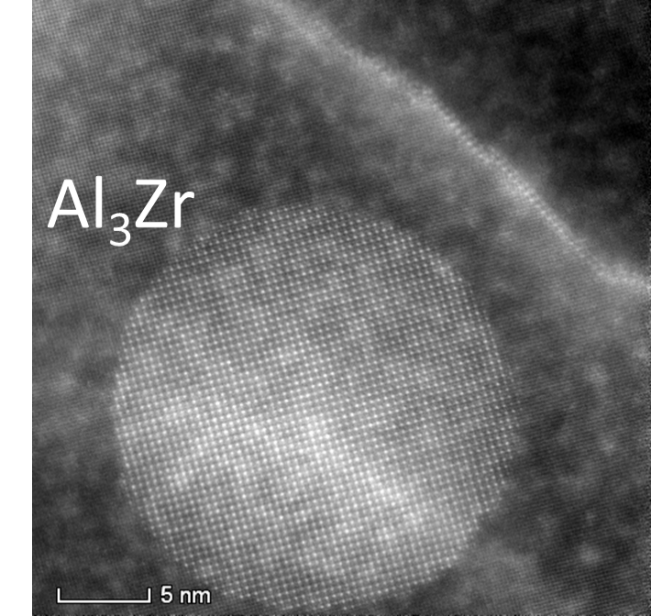
\includegraphics[height=20cm]{figs/coherent_interface_STEM}
  \tikz{
    \draw[use as bounding box] (0,0) rectangle (0,0);
    \node at (-13.05,13.1) {\color{white}\scalebox{1.2}{\huge-L1\textsubscript{2}}};
    \node[left] at (0,19) {\color{white}\scalebox{1.2}{\huge S-TEM}};
  }\\
  
\includegraphics[height=20cm]{figs/structures}
\end{multicols}
}


\posterBox{1}(0,11.167189){Methods}{  
  \begin{itemize}
    \item First principles \alert{Density Functional Theory} calculations\\ as implemented in Vienna Ab initio Simulation Package \cite{Kresse1996-gt, Kresse1996-tg}
    \tikz{
      \draw[use as bounding box] (0,0) rectangle (0,0);
      \node at (4,0) {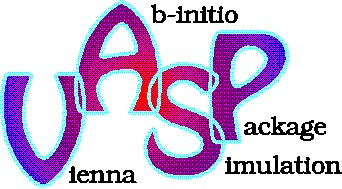
\includegraphics[width=7cm]{figs/vasp_logo}};
    }
    \item PAW enabled pseudopotentials \cite{Kresse1999-if}
    \item GGA-PBE for the exchange-correlation effects \cite{Perdew1996-vd}\vspace*{-1eX}
    \setlength{\columnsep}{2cm}
    \begin{multicols*}{2}
      \item \alert{Differences} between \alert{structures} in\\ the stacking of the (001) Zr-Al planes:
      \begin{itemize}
        \item L$1_2$: \quad \dots AAAAA\dots
        \item D$0_{22}$: \quad \dots ABABA\dots
        \item D$0_{23}$: \quad \dots AABBA\dots
      \end{itemize}\columnbreak
      \item \alert{alloying} approach:
      \begin{itemize}
        \item set of 16 doping elements
        \item 64 atom supercells
        \item 1 ternary substituent $\leadsto$ approx 1.5\,at.\%
      \end{itemize}
    \end{multicols*}
  \end{itemize}
}


\posterBox{1}(0,17.983726){Energy of formation}{
  \centering
  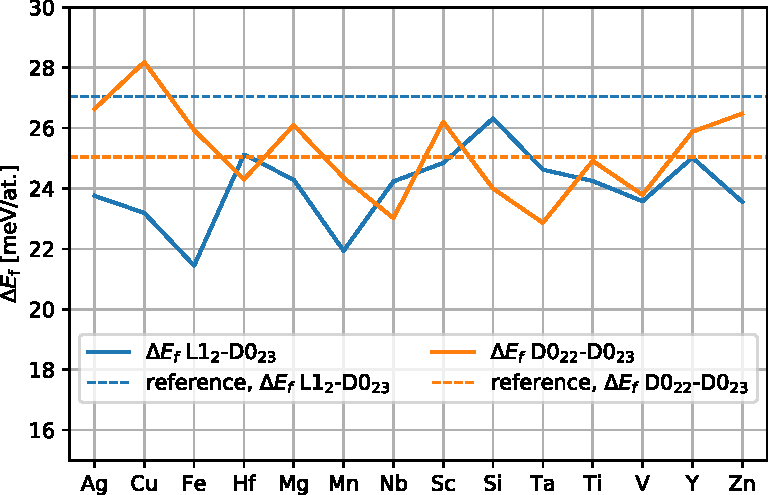
\includegraphics[width=\dhBoxTextWidth]{figs/Ef_diff}\bigskip
  \setlength{\fboxsep}{5mm}
  \framebox{\Alert{\Large $E_f(\mbox{D}0_{23}) \ll E_f(\mbox{L}1_2),\ E_f(\mbox{D}0_{22})$}}
}


\posterBox{1}(0,32.067523){Site preference}{
  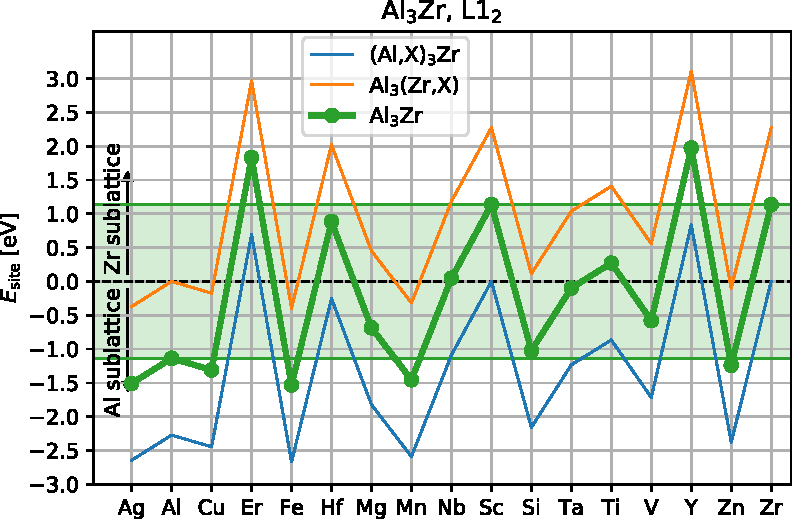
\includegraphics[width=\dhBoxTextWidth]{figs/L12_site_preference}
  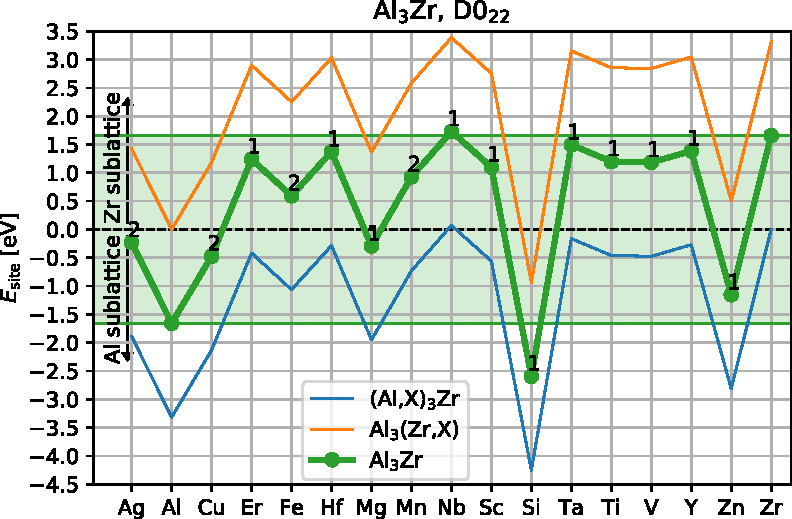
\includegraphics[width=0.5\dhBoxTextWidth]{figs/D022_site_preference}
  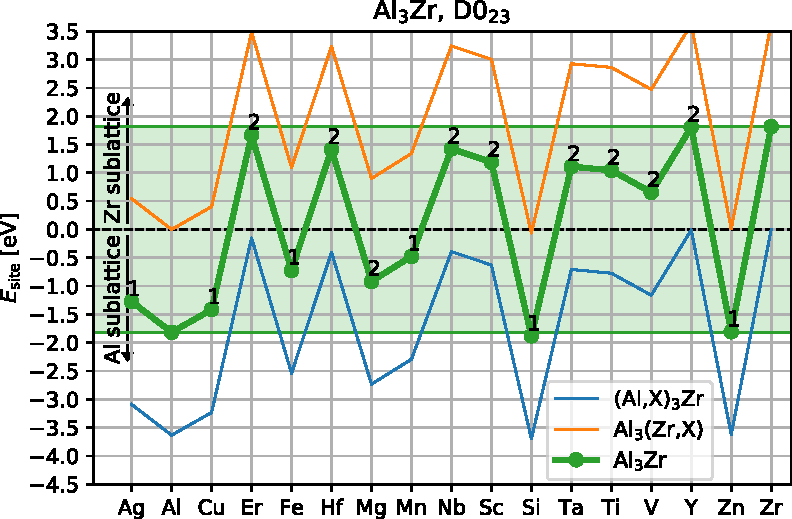
\includegraphics[width=0.5\dhBoxTextWidth]{figs/D023_site_preference}
}


\posterBox{1}(1,11.167189){Transformation barriers}{
  \begin{minipage}{0.48\dhBoxTextWidth}
    \begin{itemize}
      \item \Alert{Idea:} Increase \alert{barrier} for the \alert{AA$\to$AB stacking fault} to prevent L$1_2\to$D$0_{22}$/D$0_{23}$ transformation
    \end{itemize}\bigskip
    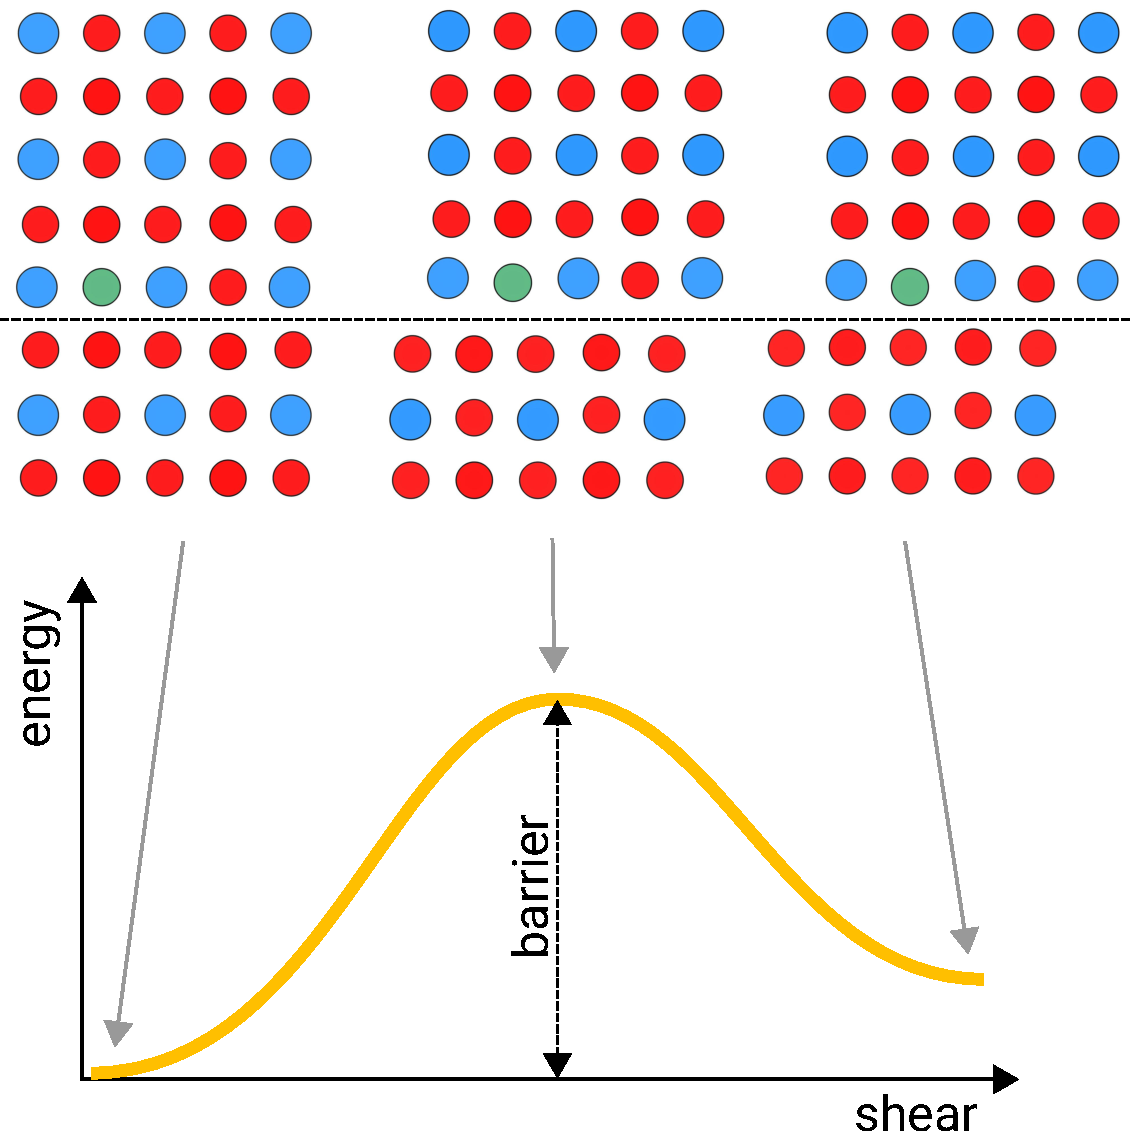
\includegraphics[width=\textwidth]{figs/barrier_schematics}
  \end{minipage}\hfill
  \begin{minipage}{0.5\dhBoxTextWidth}
    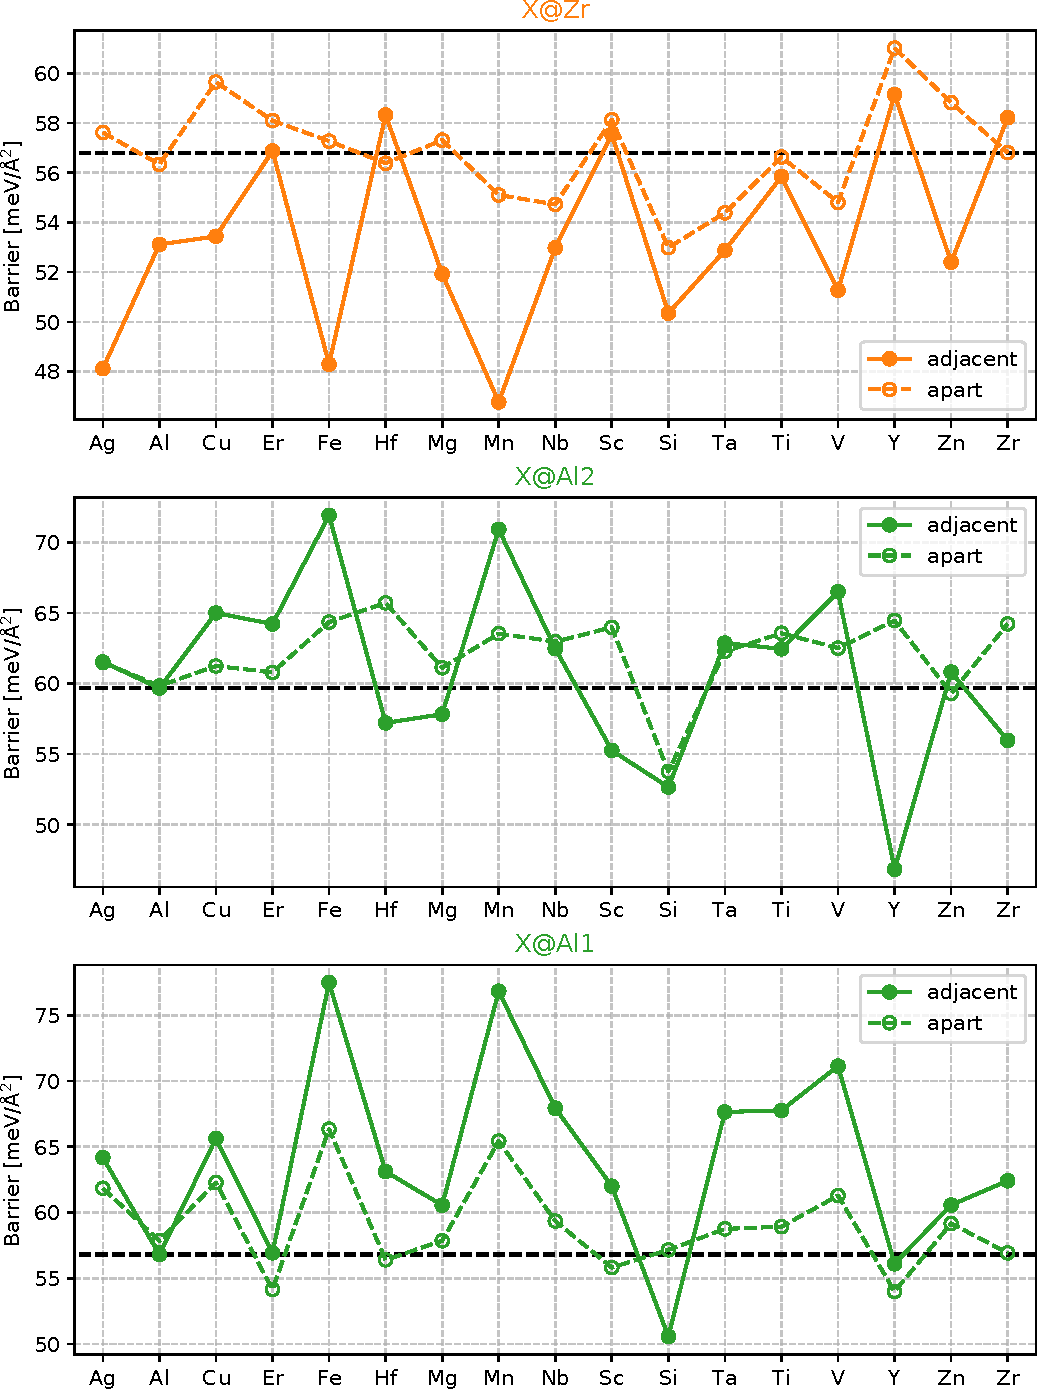
\includegraphics[width=0.5\dhBoxTextWidth]{figs/barrier}
  \end{minipage}
}


\posterBox{1}(1,24.069957){FactSage prediction of Nb solubility}{
  \begin{itemize}
    \item Calphad-based assessment (FactSage \cite{Bale2009-sa})of \alert{maximum solubility} of ternary addition in the L$1_2$ (\ce{Al3Zr}(s) phase)
    \item \Alert{Example:} Nb--Al phase diagram for fixed Zr content of 0.21\,wt.\% (0.0601\,at.\%)
  \end{itemize}
  \centering
  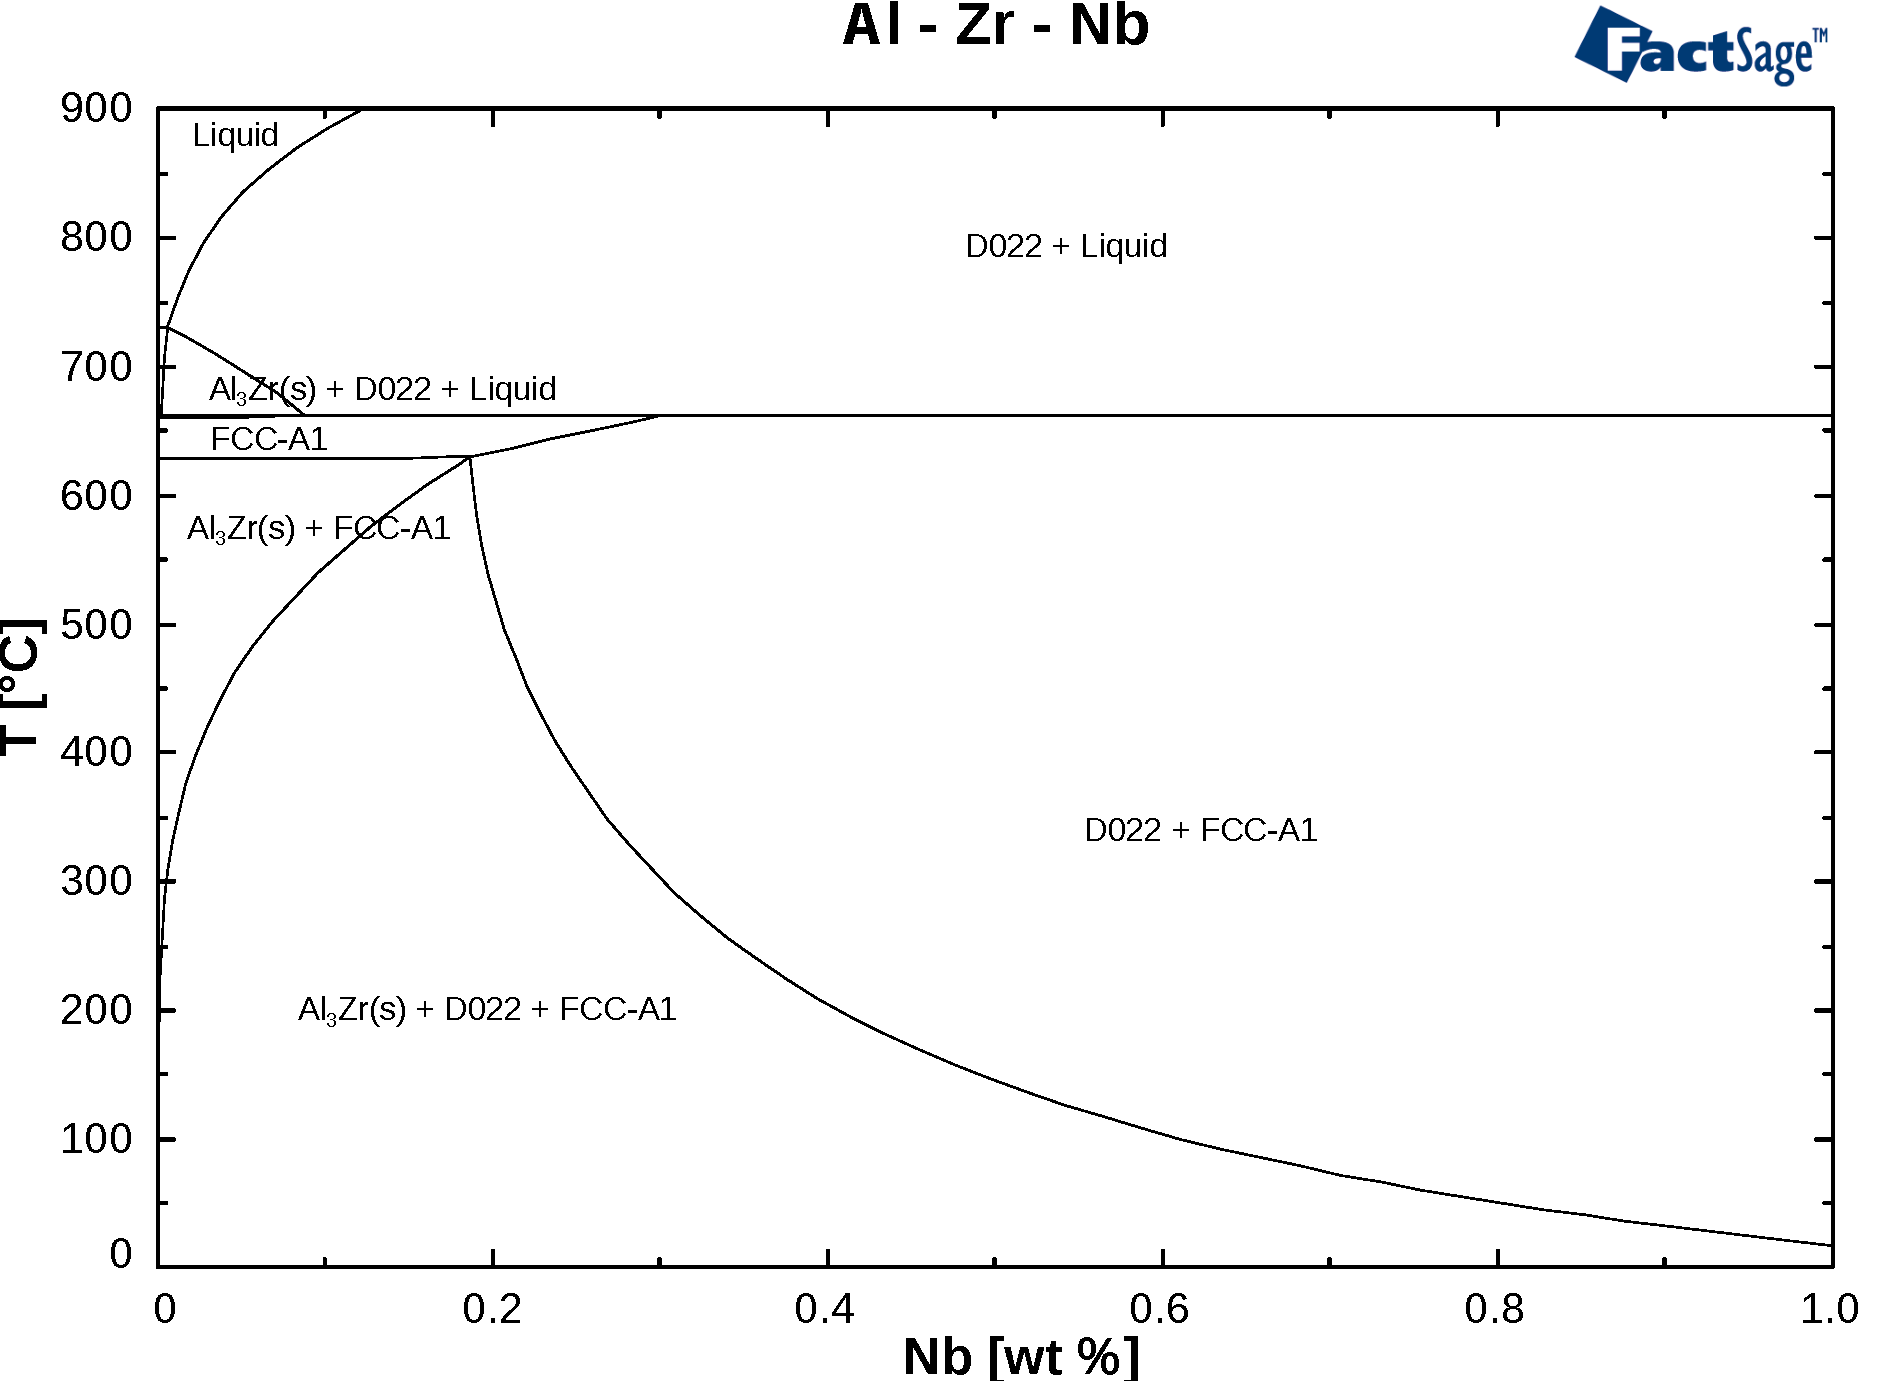
\includegraphics[width=0.985\dhBoxTextWidth]{figs/Al-Zr-Nb}
}


\posterBox{1}(1,39.833221){Experiments}{
  \begin{itemize}
    \item \Alert{Elements selected} for \alert{experimental verification} based on the modelling predictions:
    \begin{itemize}
      \item \Alert{Zr substituents}: Er, Hf, Nb, Sc, Y
      \item \Alert{Al substituents}: Ag, Cu, Mn, Zn, Si
    \end{itemize}
    \item Alloys are \alert{cast} in an inductively heated furnace to 800\,$^{\circ}$C (940\,$^{\circ}$C for Nb)
    \item \Alert{Homogenization} 15--20\,$^{\circ}$C under their respective solidus temperature for 24\,h and \alert{water-quenched}
    \item \alert{Ageing} of alloys at temperatures between 450 and 550\,$^{\circ}$C for 24\,h
    \item Microstructural analysis is carried out primarily using a \alert{S-TEM} (Talos, FEI)
  \end{itemize}
}

\posterBox*{1}(1,46.4663){References}{
  \begingroup
  \renewcommand{\section}[2]{}%
  \let\oldbibliography\thebibliography
  \renewcommand{\thebibliography}[1]{\oldbibliography{#1}
  \setlength{\itemsep}{0pt}} 
  \bibliographystyle{aipnum4-1}
  \small\bibliography{refs}
  \endgroup\vspace*{-2mm}
}  

\node[above right] at (0,0) {\parbox{\dhColumnWidth}{
  \small
  {\bfseries Acknowledgements:} The computational results presented have been achieved [in part] using the Vienna Scientific Cluster (VSC).
}};
 
\end{document}
